\begin{frame}[shrink=10]
  \begin{columns}
    \begin{column}{0.5\textwidth}
      \centering
      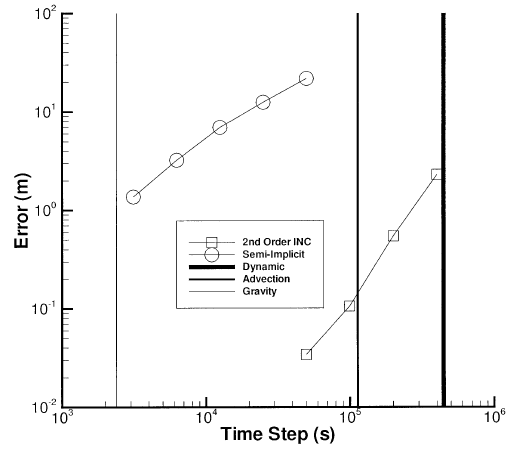
\includegraphics[width=0.78\textwidth]{figures/MousseauOceanError} \\
      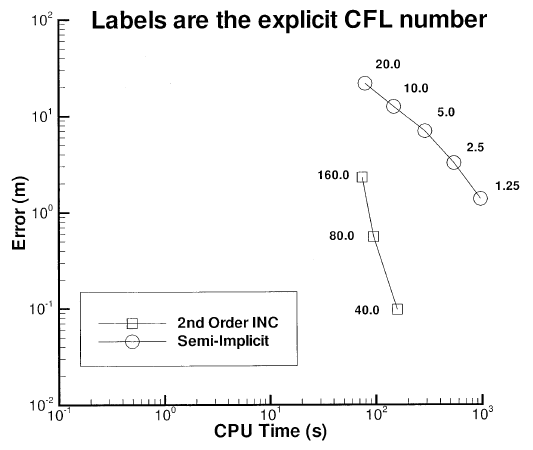
\includegraphics[width=0.78\textwidth]{figures/MousseauOceanTime} \\
      \scriptsize{Shallow water traveling vortex with Coriolis. \\ Moussau et al, 2002.}
    \end{column}
    \begin{column}{0.5\textwidth}
      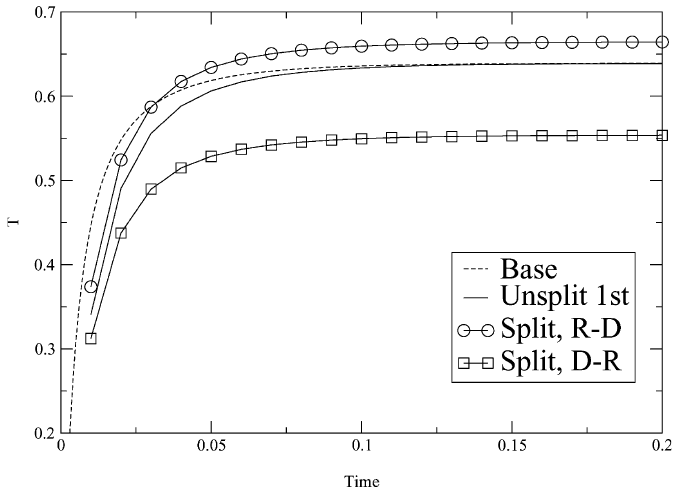
\includegraphics[width=0.78\textwidth]{figures/KnollSplittingRD} \\
      \scriptsize{Linear reaction-diffusion, split method converges to \\
        the wrong steady state . Knoll et al, 2003.}
      \begin{itemize}\small
      \item CFL too restrictive for explicit
        \begin{itemize}
        \item But hyperbolic systems do not weak scale if you care about phase
        \end{itemize}
      \item Naive semi-implicit has poor accuracy, stability, robustness
      \item Good IMEX exists, but still need to treat stiff part implicitly
      \end{itemize}
    \end{column}
  \end{columns}
\end{frame}
